\section{Existing General Purpose Platforms} 

Today's general purpose data platforms fall short of supporting secure, real-time decisions on live data. To illustrate this point, consider a movie recommendation engine as shown in Figure~\ref{fig:related}. Users logs (e.g., viewing preference, ratings) are collected via a message broker such as Kafka and stored in a distributed files system, such as HDFS or S3. A Hadoop or Spark job will periodically read these logs and train a model to capture user recommendations. Then, these models are pushed into a key value store, such as HBASE or DynamoDB, from which they are served to users. For instance, when a user logs in, the application will query the key-value store to retrieve the movie recommendations for that user. While such a key-value store can provide millisecond-level delays, this solution has several significant drawbacks:

\0
\begin{figure}[h]
  \center{
 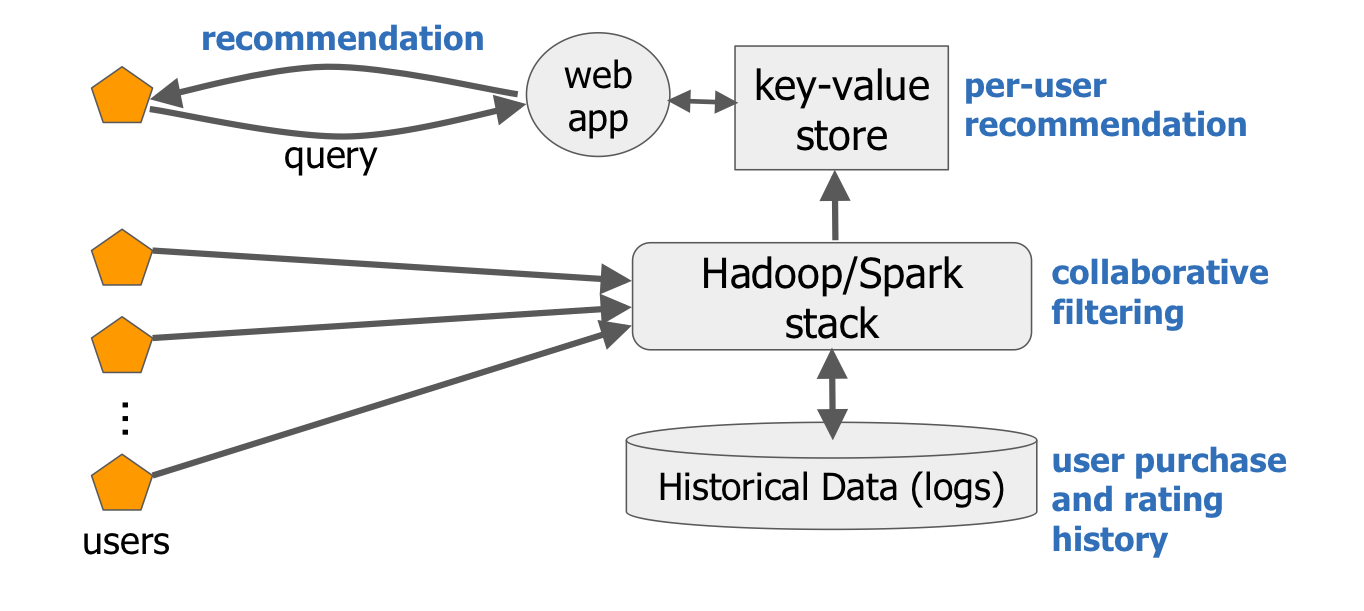
\includegraphics[scale=0.35]{figures/existing-solutions}
  }
  \vskip -.15in
  \caption{\small{The implementation of a recommendation system.}}
\label{fig:related}
\end{figure}



{\bf Simple decisions}: With a simple key-value store it is hard to support sophisticated decisions, such as ML classification or clustering. One way to support such decisions would be to pre-compute all possible decisions. Unfortunately, in general, this is infeasible due to ``the curse of dimensionality''~\cite{Agarwal14, Crankshaw15}. Another possibility would be to run non-trivial algorithms on non-trivial amounts of data. Unfortunately, this will compromise the query latency.  

{\bf Slow updates}: Typically, the intermediate representation (e.g., model) is updated hourly, or even daily. While Spark increases the update frequency it is still in the order of hours, as one needs to read data from the distributed file system, re-compute the model and push the changes to the key-value store.

{\bf Weak security}: In most existing solutions, the main security measure employed is encryption at rest or encryption over the network. The pre-processing and decision logic run with access to decrypted data and are thus vulnerable to any 3rd party attacks or to insider attacks. This is in particular troublesome when computations run on the public clouds, which is fast becoming the norm, rather than the exception. 

In the research community, two techniques are emerging as possible solutions to protect the application's integrity and user's privacy. The first is computing on encrypted data which was first proposed in the theory community~\cite{databanks78, gentry2009fully}, and then popularized in practical systems by CryptDB~\cite{cryptdb} and Mylar~\cite{mylar}. The second is leveraging hardware enclaves~\cite{IntelSGX}, which are now integrated in both Intel and ARM chips to securely run arbitrary software in untrusted environments, such as the public cloud. However, none of these techniques are perfect. While computing on encrypted data makes minimal assumptions about the hosted environment, it can support only a limited functionality on encrypted data. In contrast, hardware enclaves allow one to run arbitrary code, but they leak data if there are bugs in the trusted code running in the enclave, if untrusted code runs in the enclave, and from various side channels~\cite{SGXmemorychannel, SGXnetworkchannel}.

